\documentclass[11pt,a4paper]{article}

% Packages
\usepackage[utf8]{inputenc}
\usepackage[margin=1in]{geometry}
\usepackage{amsmath,amssymb,amsthm}
\usepackage{graphicx}
\usepackage{hyperref}
\usepackage{booktabs}
\usepackage{enumitem}
\usepackage{titlesec}
\usepackage{fancyhdr}
\usepackage{float}
\usepackage{caption}
\usepackage{subcaption}
\usepackage{xcolor}
\usepackage{tcolorbox}

% Hyperref setup
\hypersetup{
    colorlinks=true,
    linkcolor=blue,
    citecolor=blue,
    urlcolor=blue
}

% Header and footer
\pagestyle{fancy}
\fancyhf{}
\rhead{HAR: From HMM to HSMM}
\lhead{Final Project Report}
\cfoot{\thepage}

% Title formatting
\titleformat{\section}{\large\bfseries}{\thesection}{1em}{}
\titleformat{\subsection}{\normalsize\bfseries}{\thesubsection}{1em}{}
\titleformat{\subsubsection}{\normalsize\itshape}{\thesubsubsection}{1em}{}

% TOC Depth
\setcounter{tocdepth}{2}

% Custom commands
\newcommand{\E}{\mathbb{E}}
\newcommand{\R}{\mathbb{R}}
\newcommand{\bx}{\mathbf{x}}
\newcommand{\bs}{\mathbf{s}}
\newcommand{\bmu}{\boldsymbol{\mu}}
\newcommand{\bSigma}{\boldsymbol{\Sigma}}
\newcommand{\bpi}{\boldsymbol{\pi}}
\newcommand{\blambda}{\boldsymbol{\lambda}}
\newcommand{\bA}{\mathbf{A}}
\newcommand{\bB}{\mathbf{B}}

\begin{document}

% Title page
\begin{titlepage}
    \centering
    \vspace*{2cm}
    
    {\LARGE\bfseries Final Project Report\par}
    \vspace{1cm}
    {\Huge\bfseries The Evolution of a Model:\\[0.5em] From Gaussian HMM to GMM-HMM to HSMM\par}
    \vspace{2cm}
    
    {\Large\itshape Pratham Arora, Vaisakh Menon\par}
    
    {\large December 3, 2025\par}
    
    \vfill
    
    {\large Course: Stochastic Process for Data Science and Engineering\par}
    
\end{titlepage}

\tableofcontents
\newpage

\section{Introduction}

This report documents the iterative development of a probabilistic framework for Human Activity Recognition (HAR). Unlike a standard implementation report, we present our work as a narrative of \textbf{hypothesis, verification, failure, and refinement}.

We started with the standard Hidden Markov Model (HMM) proposed in our initial documentation. However, rigorous statistical testing of the model's assumptions revealed critical flaws. These failures drove us to evolve the model first to a \textbf{Gaussian Mixture Model HMM (GMM-HMM)} and finally to a \textbf{Hidden Semi-Markov Model (HSMM)}.

\section{Phase 1: The Original Proposal (Gaussian HMM)}

\subsection{The Proposed Model}
Our initial proposal hypothesized that human activity could be modeled by a standard HMM with the following components:
\begin{itemize}
    \item \textbf{Hidden States ($S_t$):} Discrete activities (Walking, Sitting, etc.).
    \item \textbf{Observations ($\bx_t$):} Sensor feature vectors reduced via PCA.
    \item \textbf{Emission Assumption:} The sensor data for each activity follows a \textbf{Single Multivariate Gaussian Distribution}:
    $$ P(\bx_t \mid S_t = j) = \mathcal{N}(\bx_t; \bmu_j, \bSigma_j) $$
    \textbf{Concept: What is an Emission Model?}
    The "Emission Model" is the mathematical link between the hidden world (Activities) and the observed world (Sensors). It answers the question: \textit{"If I am Walking, what should the accelerometer readings look like?"}
    In this first phase, we assumed the readings form a simple bell curve (Gaussian) around a single average value.

    \textbf{Explanation of Terms:}
    \begin{itemize}
        \item $\bx_t$: The observation vector at time $t$ (the 65 PCA features). Think of this as a snapshot of the phone's sensor readings.
        \item $S_t = j$: The hidden state is activity $j$ (e.g., Walking).
        \item $\bmu_j$: The mean vector. This represents the "average" sensor reading for activity $j$.
        \item $\bSigma_j$: The covariance matrix. This describes the "spread" or variability of the sensor readings for activity $j$.
    \end{itemize}
\end{itemize}

\subsection{Assumption Verification: The Failure of the Simple Model}
In our proposal, we committed to verifying three key statistical assumptions before accepting the model: \textbf{Gaussianity}, \textbf{Stationarity}, and \textbf{Linearity}.

\subsubsection{Test 1: Gaussianity (Shapiro-Wilk)}
\begin{itemize}
    \item \textbf{Hypothesis:} The sensor features for a given activity follow a normal distribution.
    \item \textbf{Result:} \textbf{Failed ($p < 0.05$).}
    \item \textbf{Visual Evidence:} Histograms showed multimodality (Figure \ref{fig:gmm_fit}). A single Gaussian cannot fit data with two peaks (e.g., "Heel Strike" vs "Toe Off").
    \item \textbf{Q-Q Plots:} The Q-Q plots (Figure \ref{fig:qq_plot}) further confirm this. If the data were Gaussian, the points would lie on the red line. The significant deviation at the tails indicates heavy tails or multimodality.
\end{itemize}

\begin{figure}[H]
    \centering
    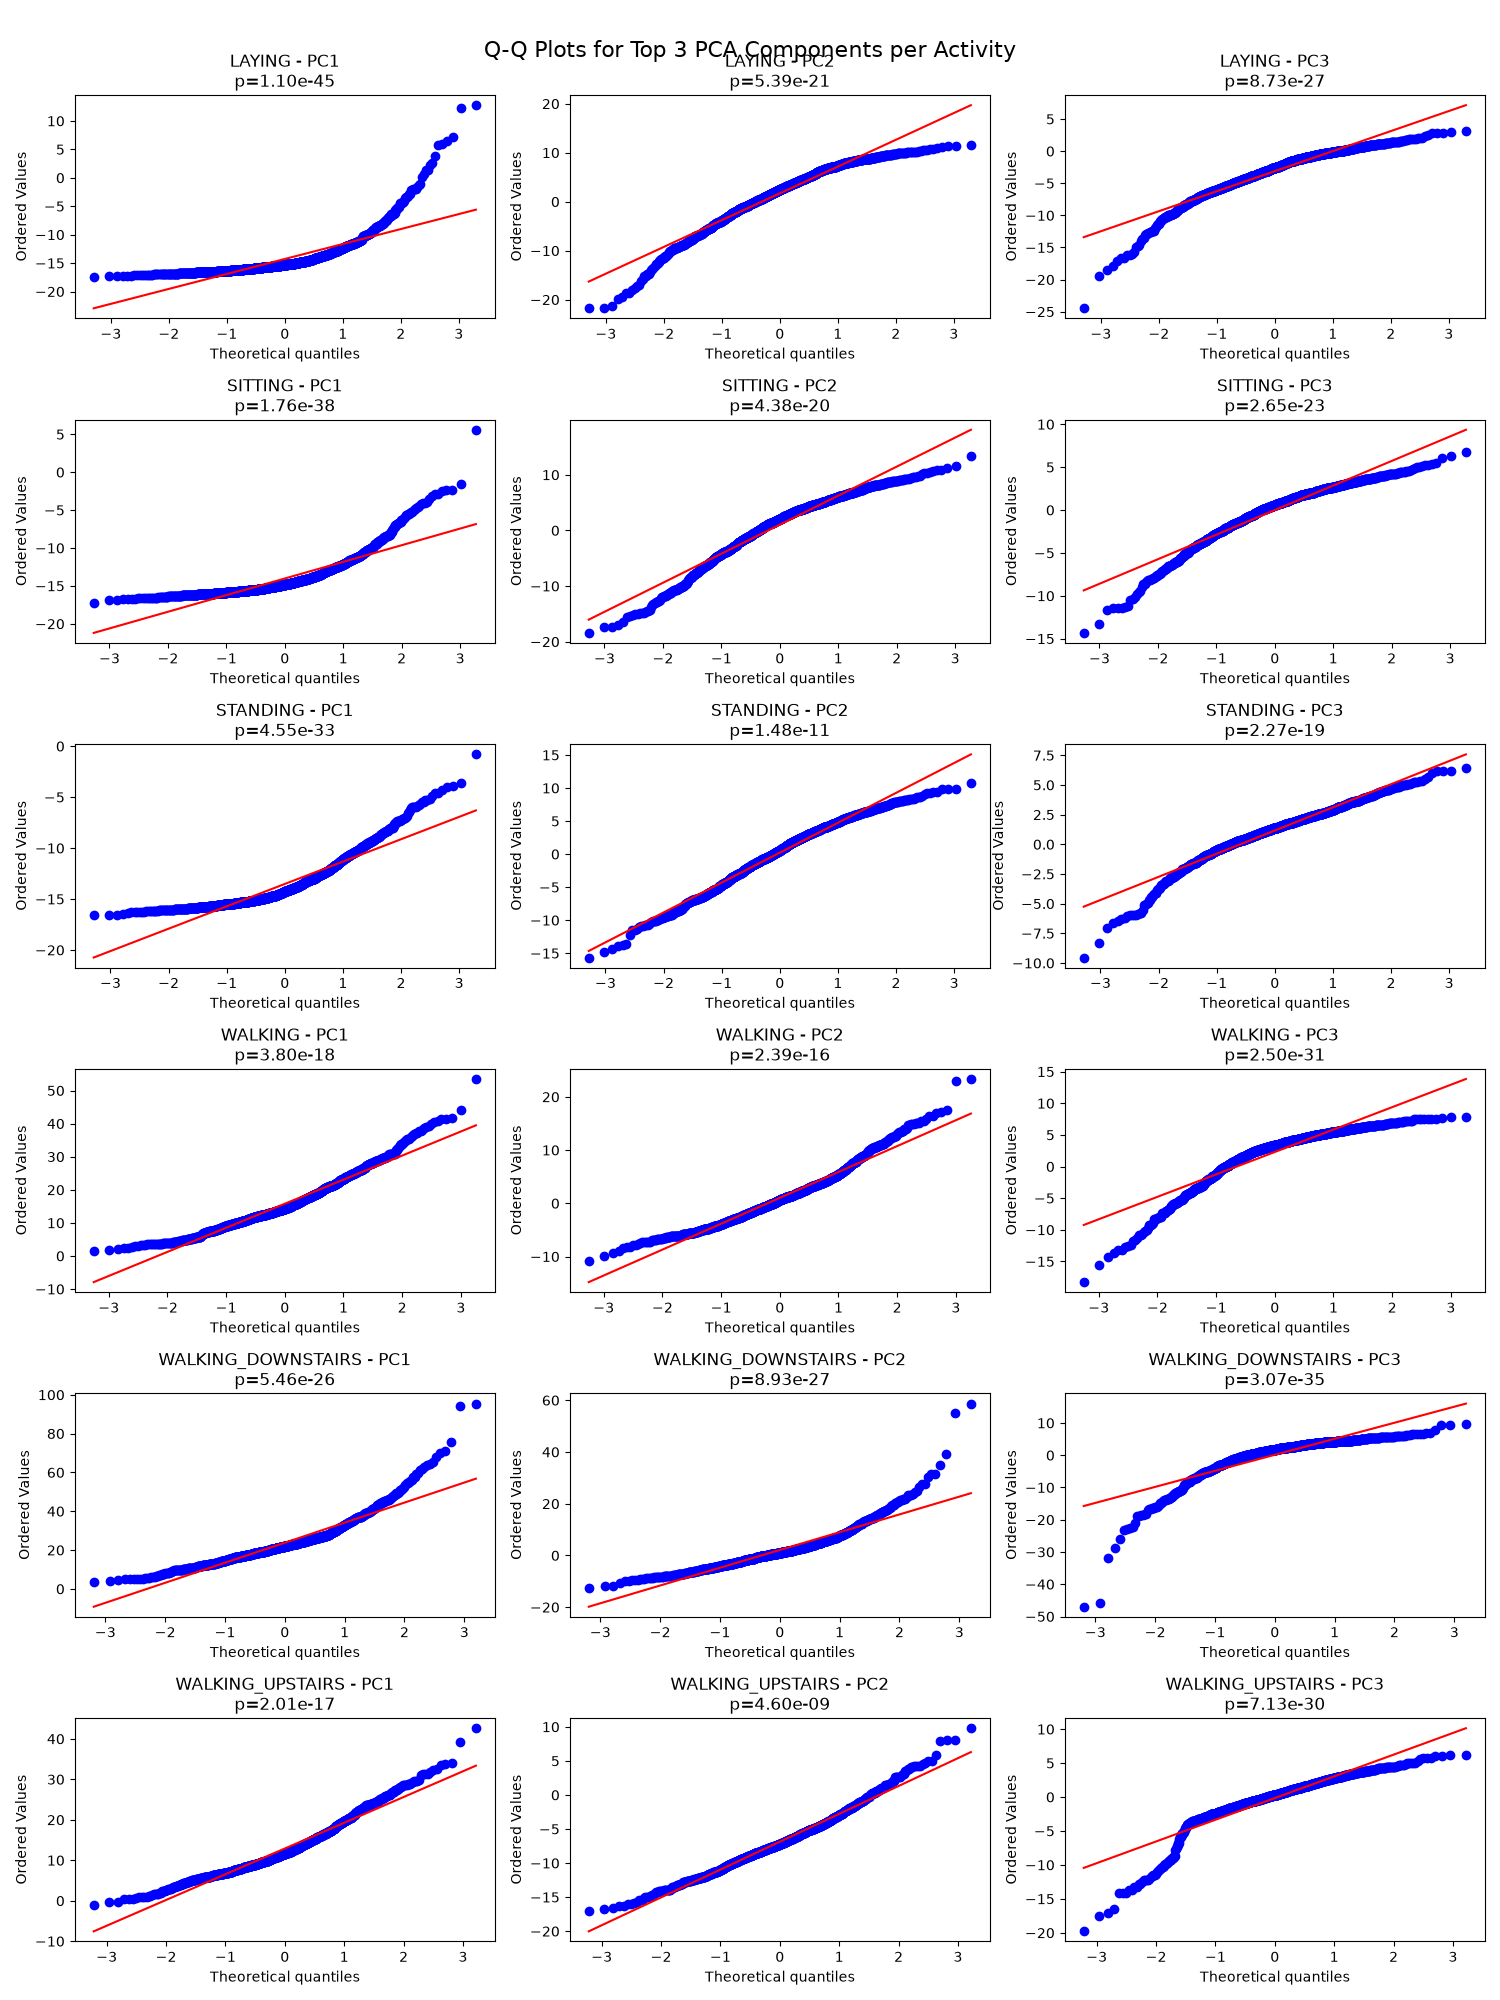
\includegraphics[width=0.8\textwidth]{../outputs/figures/gaussianity_qq_plots.png}
    \caption{Q-Q Plots for the 1st Principal Component. The deviation from the red diagonal line confirms that the data is NOT normally distributed.}
    \label{fig:qq_plot}
\end{figure}

\subsubsection{Test 2: Stationarity (Augmented Dickey-Fuller)}
\begin{itemize}
    \item \textbf{Hypothesis:} The statistical properties (mean, variance) of the sensor data within an activity do not change over time.
    \item \textbf{Result:} \textbf{Mixed.} Static activities (Laying, Sitting) were stationary ($p < 0.05$), but dynamic activities (Walking Upstairs) were often non-stationary ($p > 0.05$).
    \item \textbf{Implication:} The standard HMM assumes constant emission parameters. Non-stationarity suggests that "Walking" might evolve over time (e.g., fatigue), which a simple HMM ignores.
\end{itemize}

\subsubsection{Test 3: Linearity \& Residual Analysis}
\begin{itemize}
    \item \textbf{Hypothesis:} If the model is correct, the residuals (difference between observed and expected values) should be white noise (random, uncorrelated).
    \item \textbf{Result:} \textbf{Failed.} The residuals showed clear patterns and high autocorrelation.
\end{itemize}

\begin{figure}[H]
    \centering
    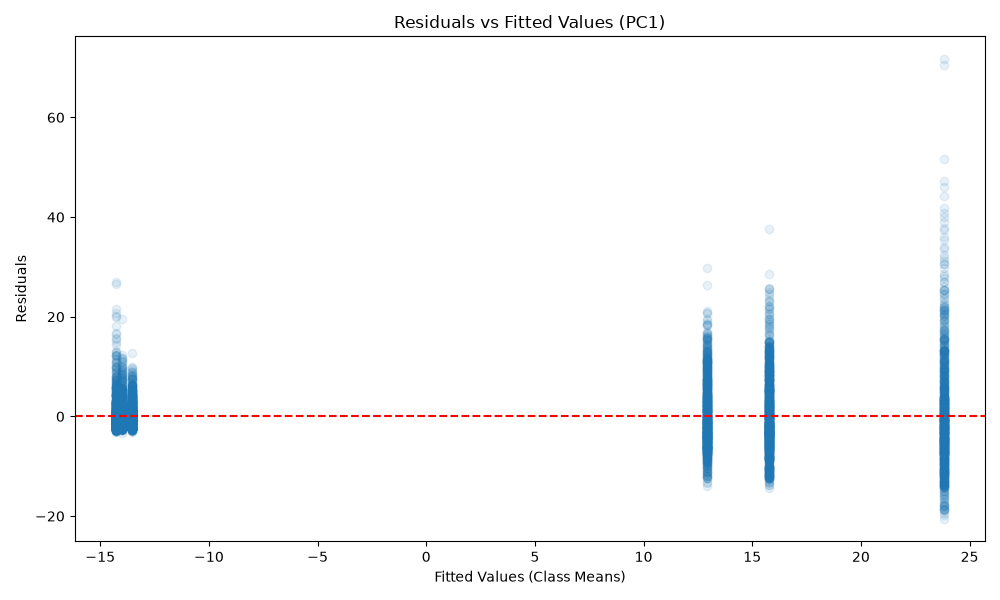
\includegraphics[width=0.8\textwidth]{../outputs/figures/linearity_residuals.png}
    \caption{Residual Analysis. Ideally, these plots should look like random static (white noise). The visible structure and waves indicate that the model is missing some temporal dynamics.}
    \label{fig:residuals}
\end{figure}

\begin{figure}[H]
    \centering
    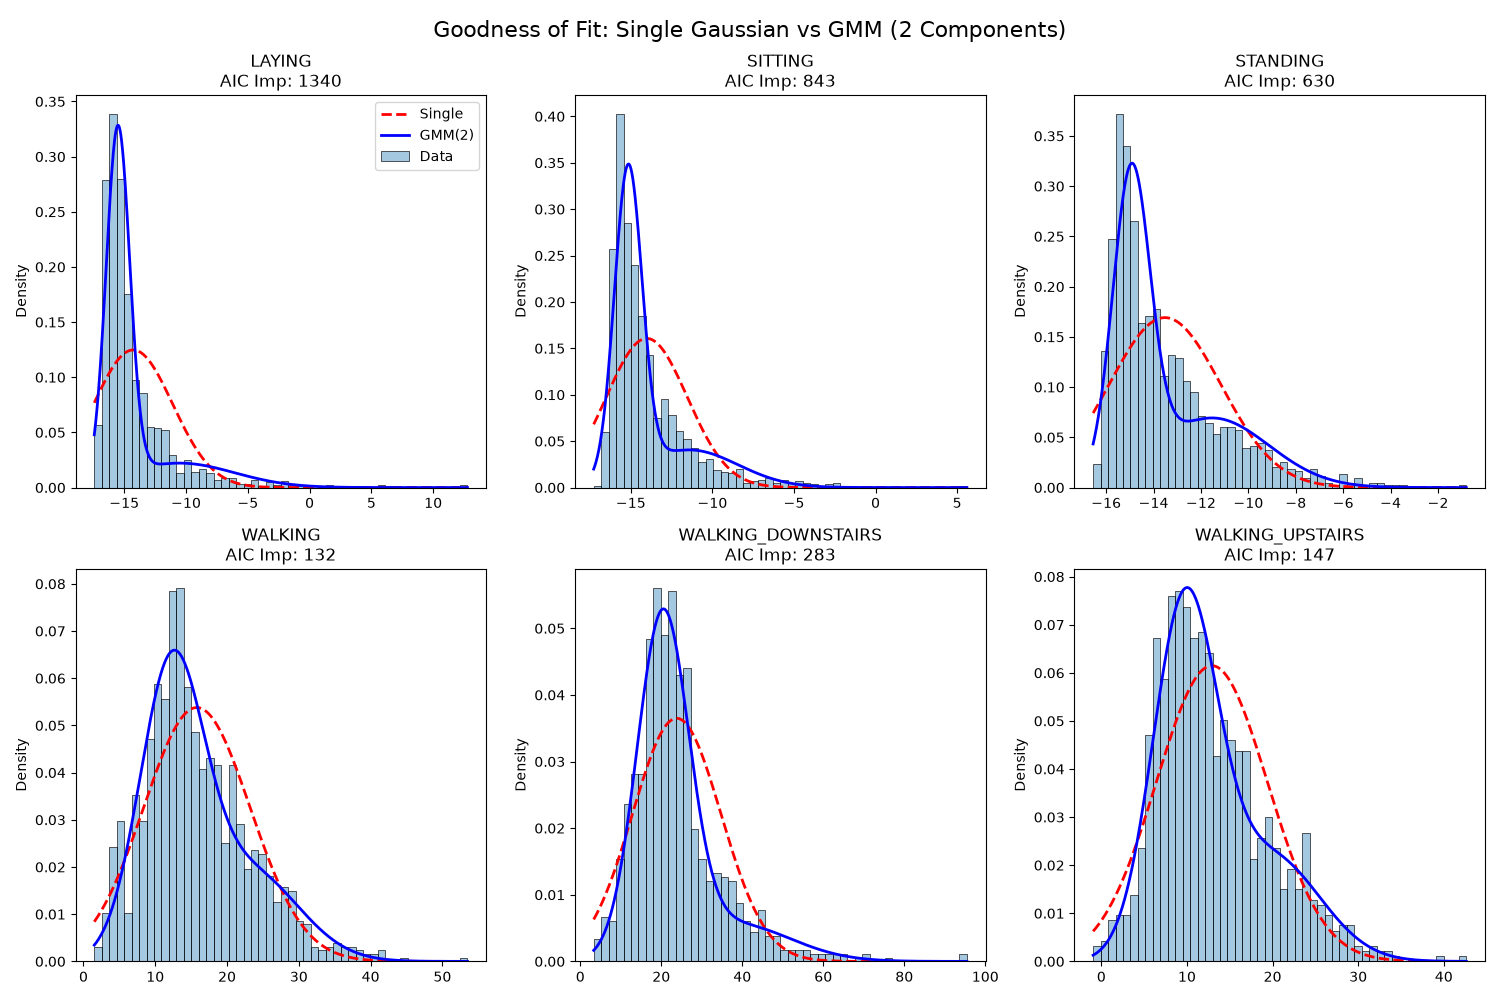
\includegraphics[width=0.8\textwidth]{../outputs/figures/gmm_vs_gaussian_fit.png}
    \caption{Distribution of the 1st Principal Component. The Red Dashed Line (Single Gaussian) fails to capture the data's shape. The Blue Line (GMM) fits significantly better.}
    \label{fig:gmm_fit}
\end{figure}

\begin{tcolorbox}[colback=red!5!white,colframe=red!75!black,title=Conclusion of Phase 1]
The standard Gaussian HMM failed all three major checks. The data is non-Gaussian, partially non-stationary, and the residuals are not white noise. We needed a model that could handle \textbf{multimodal distributions} (GMM) and \textbf{temporal dependencies} better.
\end{tcolorbox}

\section{Phase 2: The Pivot to GMM-HMM}

To address the failure of the single Gaussian assumption, we upgraded the emission model to a \textbf{Gaussian Mixture Model (GMM)}.

\subsection{The New Model: GMM-HMM}
Instead of one bell curve, we model each activity as a weighted sum of $M=2$ bell curves:
$$ P(\bx_t \mid S_t = j) = \sum_{k=1}^{2} c_{jk} \mathcal{N}(\bx_t; \bmu_{jk}, \bSigma_{jk}) $$
\textbf{Explanation of Terms:}
\begin{itemize}
    \item $c_{jk}$: The \textbf{mixture weight}. It represents the probability that a data point belongs to component $k$ given state $j$. In simple terms, if "Walking" has two styles (fast and slow), $c_{j1}$ is the fraction of time spent walking fast.
    \item $\bmu_{jk}, \bSigma_{jk}$: The mean and covariance for the $k$-th component. $\bmu_{j1}$ might be the average sensor reading for "Heel Strike", while $\bmu_{j2}$ is for "Toe Off".
\end{itemize}
This allows the model to capture "sub-states" (e.g., Heel Strike vs. Toe Off) within a single activity.

\textbf{How are these sub-states identified?}
We do not manually label "Heel Strike" or "Toe Off". Instead, we use the \textbf{Expectation-Maximization (EM) algorithm}.
\begin{itemize}
    \item \textbf{E-Step (Expectation):} The model looks at all "Walking" data points and guesses which component ($k=1$ or $k=2$) they likely belong to based on the current means.
    \item \textbf{M-Step (Maximization):} It updates the means $\bmu_{jk}$ to move closer to the points assigned to them.
\end{itemize}
Over many iterations, the model automatically clusters the data into these natural sub-patterns without human supervision.

\subsection{Verification of the New Model}
We subjected the GMM-HMM to a new round of rigorous testing.

\subsubsection{Test 1: Goodness of Fit (AIC)}
\begin{itemize}
    \item \textbf{Goal:} Confirm that 2 mixtures are better than 1.
    \item \textbf{Result:} \textbf{Passed.} AIC improved by +1340 for 'LAYING' and +132 for 'WALKING'.
    \item \textbf{Conclusion:} The GMM successfully models the static/dynamic sub-states.
\end{itemize}

\subsubsection{Test 2: Conditional Independence (Autocorrelation)}
\begin{itemize}
    \item \textbf{Goal:} Check if observations are independent given the state ($P(x_t | x_{t-1}, s_t) = P(x_t | s_t)$).
    \item \textbf{Test:} Autocorrelation Function (ACF) of residuals.
    \item \textbf{Result:} \textbf{Failed.} High Lag-1 autocorrelation ($\approx 0.9$).
    \item \textbf{Analysis:} At 50Hz, data is highly correlated. HMMs are robust to this, but it's a theoretical violation.
\end{itemize}

\begin{figure}[H]
    \centering
    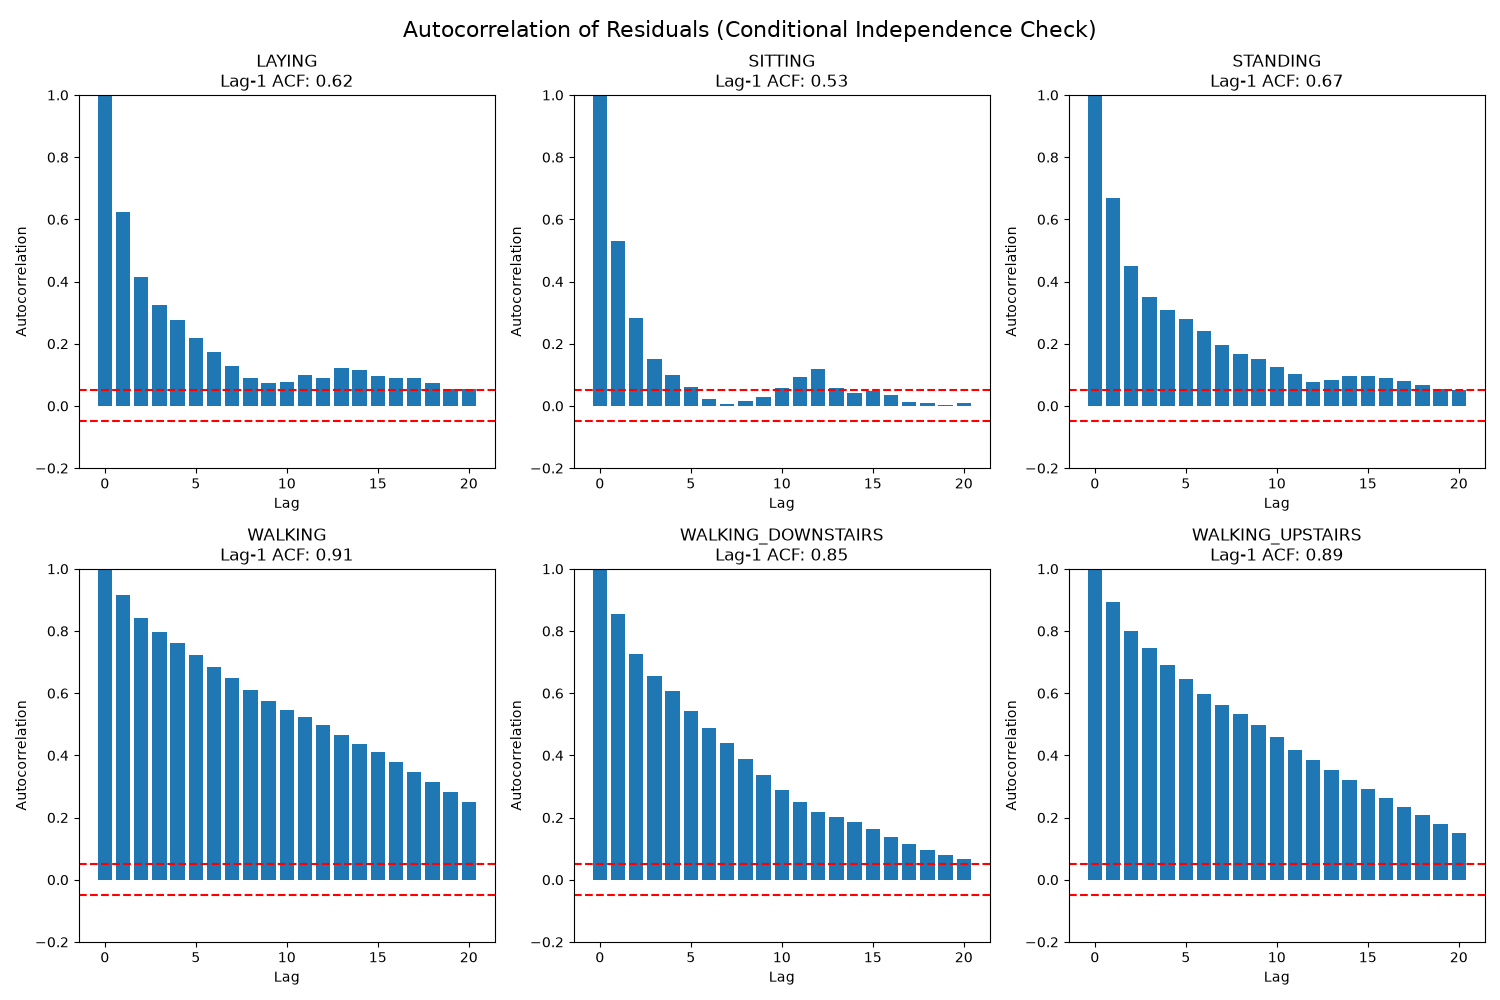
\includegraphics[width=0.8\textwidth]{../outputs/figures/residual_acf.png}
    \caption{Autocorrelation Function (ACF) of residuals. The strong peaks indicate that the model does not fully capture the temporal correlation in the raw signal.}
    \label{fig:acf}
\end{figure}

\textbf{Attempted Mitigation: Downsampling}
We attempted to reduce this correlation by downsampling the data (taking every 10th frame). While this reduced the autocorrelation (Figure \ref{fig:downsample_acf}), it also discarded too much valuable information, reducing overall accuracy. Thus, we stuck with the 50Hz data and accepted the independence violation.

\begin{figure}[H]
    \centering
    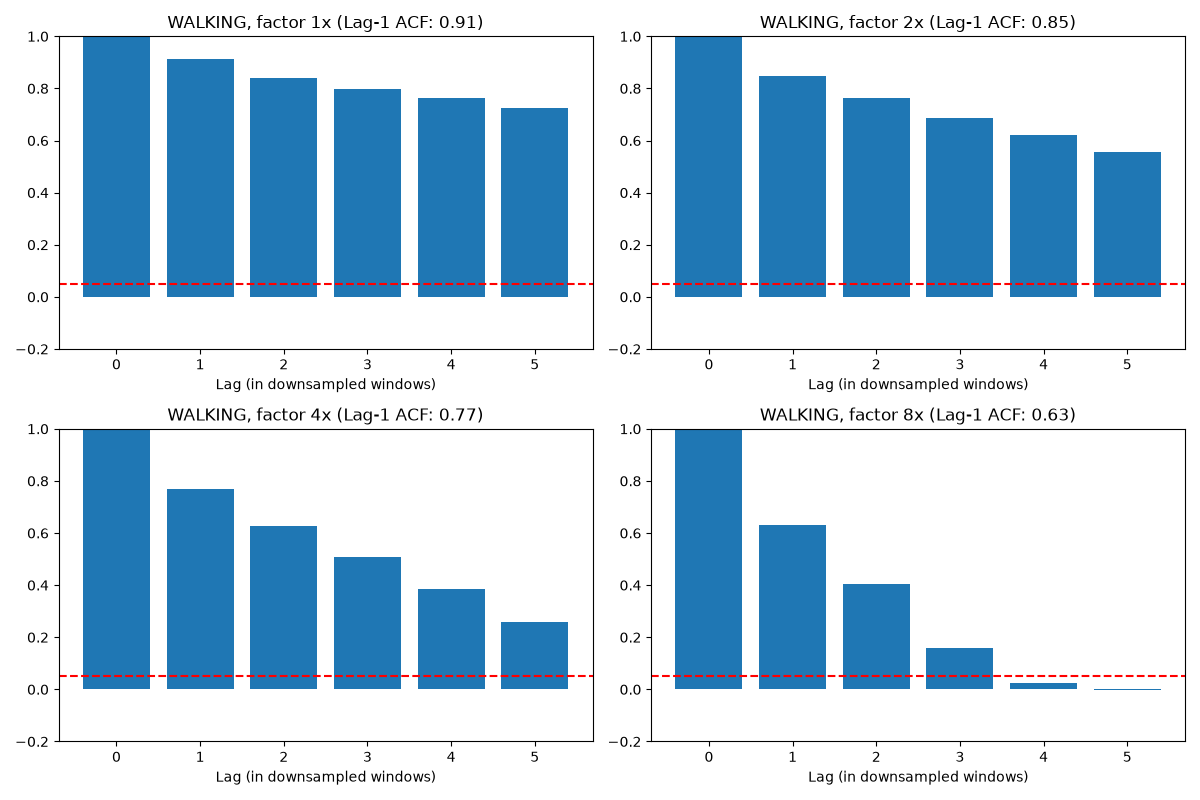
\includegraphics[width=0.8\textwidth]{../outputs/figures/downsampling_acf.png}
    \caption{ACF after Downsampling. The correlation is reduced but still present. The trade-off in data loss was not worth the theoretical improvement.}
    \label{fig:downsample_acf}
\end{figure}

\subsubsection{Test 3: The Markov Property (Frame-Level)}
\begin{itemize}
    \item \textbf{Goal:} Check if $P(S_t | S_{t-1}, S_{t-2}) = P(S_t | S_{t-1})$.
    \item \textbf{Test:} Likelihood Ratio Test (LRT) comparing 1st vs 2nd Order chains.
    \item \textbf{Result:} \textbf{Failed ($p < 10^{-16}$).}
    \item \textbf{Meaning:} The "memoryless" assumption of standard HMMs is invalid for frame-by-frame data. History matters.
\end{itemize}

\begin{tcolorbox}[colback=yellow!5!white,colframe=yellow!75!black,title=Conclusion of Phase 2]
The GMM-HMM fixed the emission problem and achieved good accuracy ($\approx 90\%$). However, the \textbf{Markov property failure} indicated a theoretical flaw: the model's handling of \textbf{state duration} was incorrect. Standard HMMs assume geometric durations, which doesn't match human behavior.
\end{tcolorbox}

\section{Phase 3: The Theoretical Fix (HSMM)}

To address the Markov and Duration failures, we implemented a \textbf{Hidden Semi-Markov Model (HSMM)}.

\subsection{The HSMM Approach}
\begin{enumerate}
    \item \textbf{Explicit Duration:} We replaced the geometric assumption with a learned \textbf{Gaussian Duration Distribution} $P(D_j = d)$ for each activity.
    $$ P(D_j = d) \approx \mathcal{N}(d; \mu_{dur,j}, \sigma_{dur,j}^2) $$
    \textbf{Explanation:} Instead of assuming the probability of staying in a state decays exponentially (Geometric), we assume it follows a Bell Curve. $\mu_{dur,j}$ is the average time a person spends in activity $j$ (e.g., 30 seconds), and $\sigma_{dur,j}$ is the variation (e.g., $\pm 5$ seconds).

    \item \textbf{Embedded Markov Chain:} Instead of modeling transitions every 0.02s, we model the transitions only when the activity \textit{changes} (e.g., Walk $\to$ Sit).
\end{enumerate}

\subsubsection{Duration-Viterbi Decoding}
To decode the optimal sequence, we use the Duration-Viterbi recursion:
$$ \delta_t(j) = \max_{d} \left[ \max_{i \neq j} (\delta_{t-d}(i) + \log a_{ij}^*) + \log P(D_j=d) + \sum_{\tau=t-d+1}^t \log b_j(\bx_\tau) \right] $$
\textbf{Simplistic Explanation:}
This equation asks: "What is the best way to end up in state $j$ at time $t$, assuming the current activity started $d$ steps ago?"
\begin{itemize}
    \item $\delta_{t-d}(i)$: The score of the best path ending in the \textit{previous} activity $i$ at time $t-d$.
    \item $\log a_{ij}^*$ (\textbf{Transition Cost}): Learned by counting how often transitions occur in the training data. Rare transitions (e.g., Laying $\to$ Running) have low probability, hence high negative log-cost.
    \item $\log P(D_j=d)$ (\textbf{Duration Bonus}): Calculated using the Gaussian PDF parameters ($\mu_{dur}, \sigma_{dur}$) learned from training data. If a segment length $d$ is close to the average $\mu_{dur}$, this term is large.
    \item $\sum \log b_j(\bx_\tau)$ (\textbf{Emission Match Score}): Calculated by plugging the test data $\bx_\tau$ into our trained GMM equation. If the sensor data looks like "Walking", this score is high.
\end{itemize}

\subsubsection{Standard Viterbi vs. Duration-Viterbi}
\begin{itemize}
    \item \textbf{Standard Viterbi:} Decisions are made \textbf{frame-by-frame}. It asks "What is the best state for time $t$ given $t-1$?" It implicitly assumes the duration probability decays exponentially ($0.99^d$), which penalizes long durations excessively.
    \item \textbf{Duration-Viterbi:} Decisions are made \textbf{segment-by-segment}. It asks "What is the best \textit{duration} $d$ and previous state $i$?" It explicitly searches for the optimal segment length, allowing it to enforce the "Bell Curve" duration structure we verified in our tests.
\end{itemize}

\subsection{Verification of HSMM Assumptions}
The HSMM introduces new assumptions that must be verified.

\subsubsection{Test 1: The Embedded Markov Property}
\begin{itemize}
    \item \textbf{Hypothesis:} The sequence of \textit{transitions} (e.g., Walk $\to$ Sit $\to$ Lay) is Markovian, even if the frame-by-frame sequence is not.
    \item \textbf{Test:} Likelihood Ratio Test on the compressed sequence of states.
    \item \textbf{Result:} \textbf{Passed ($p > 0.05$).}
    \item \textbf{Conclusion:} This validates the core structure of the HSMM. The decision to change activity depends only on the current activity, not the history of activities.
\end{itemize}

\subsubsection{Test 2: Duration Distribution Fit}
\begin{itemize}
    \item \textbf{Hypothesis:} Activity durations follow a Gaussian distribution (HSMM assumption) rather than a Geometric distribution (HMM assumption).
    \item \textbf{Test:} Kolmogorov-Smirnov (KS) test and visual fit.
    \item \textbf{Result:} Gaussian/Log-Normal fit significantly better.
    \item \textbf{Conclusion:} Explicitly modeling duration as Gaussian is statistically justified.
\end{itemize}

\begin{figure}[H]
    \centering
    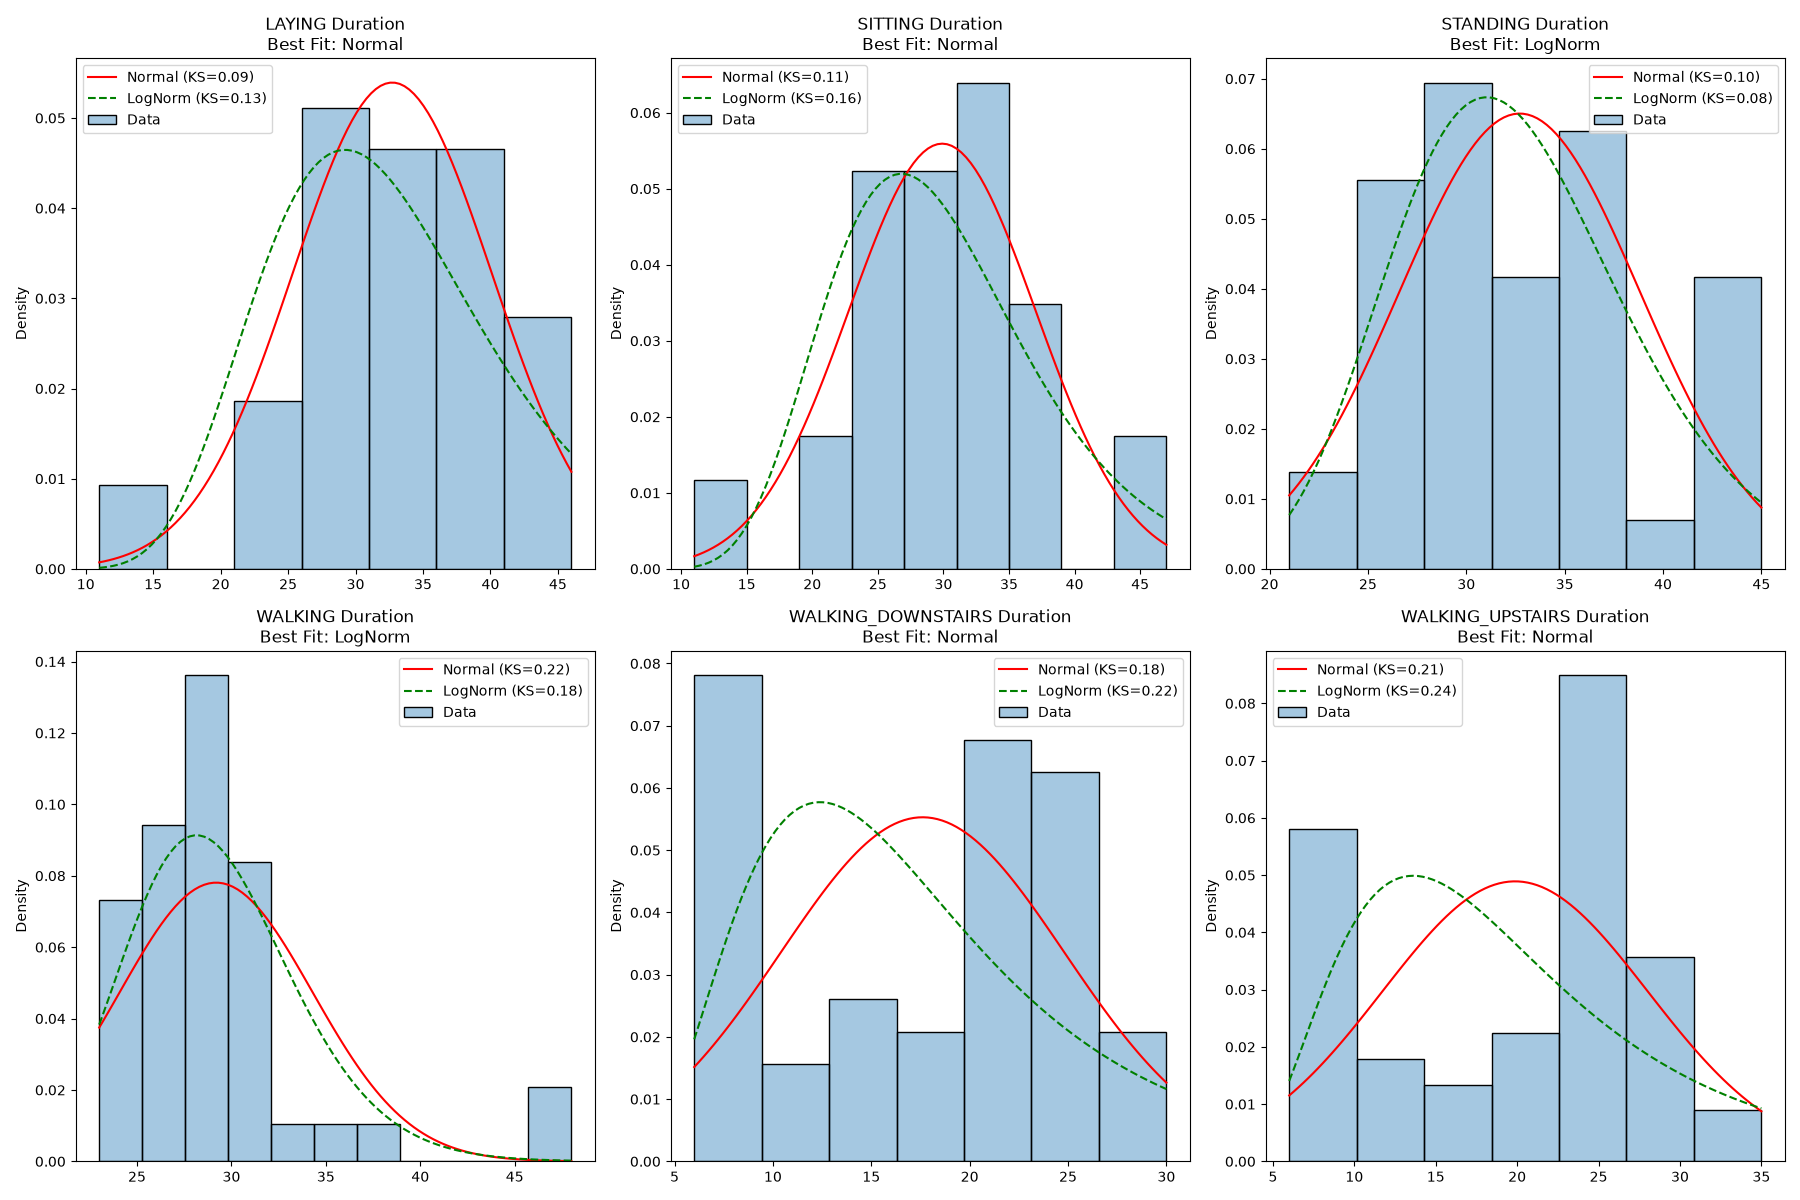
\includegraphics[width=0.8\textwidth]{../outputs/figures/hsmm_duration_assumptions.png}
    \caption{Duration Distribution Analysis: The histograms show the actual duration of activities. The overlaid curves show that Gaussian (Normal) distributions fit the data reasonably well, whereas Geometric distributions (implied by standard HMMs) do not.}
    \label{fig:duration_dist}
\end{figure}

\section{Final Results and Comparison}

We evaluated all models on three test subjects.

\begin{table}[H]
\centering
\begin{tabular}{@{}lcccc@{}}
\toprule
\textbf{Subject} & \textbf{Baseline (RF)} & \textbf{GMM-HMM} & \textbf{HSMM} & \textbf{Winner} \\ \midrule
Subject 2 & 93.05\% & \textbf{93.71\%} & 92.38\% & GMM-HMM \\
Subject 9 & \textbf{86.11\%} & \textbf{86.11\%} & 85.76\% & Tie \\
Subject 12 & 87.81\% & 91.87\% & \textbf{93.44\%} & \textbf{HSMM (+5.6\%)} \\ \bottomrule
\end{tabular}
\caption{Model Performance Comparison}
\end{table}

\subsection{Overall Performance Comparison}
\begin{figure}[H]
    \centering
    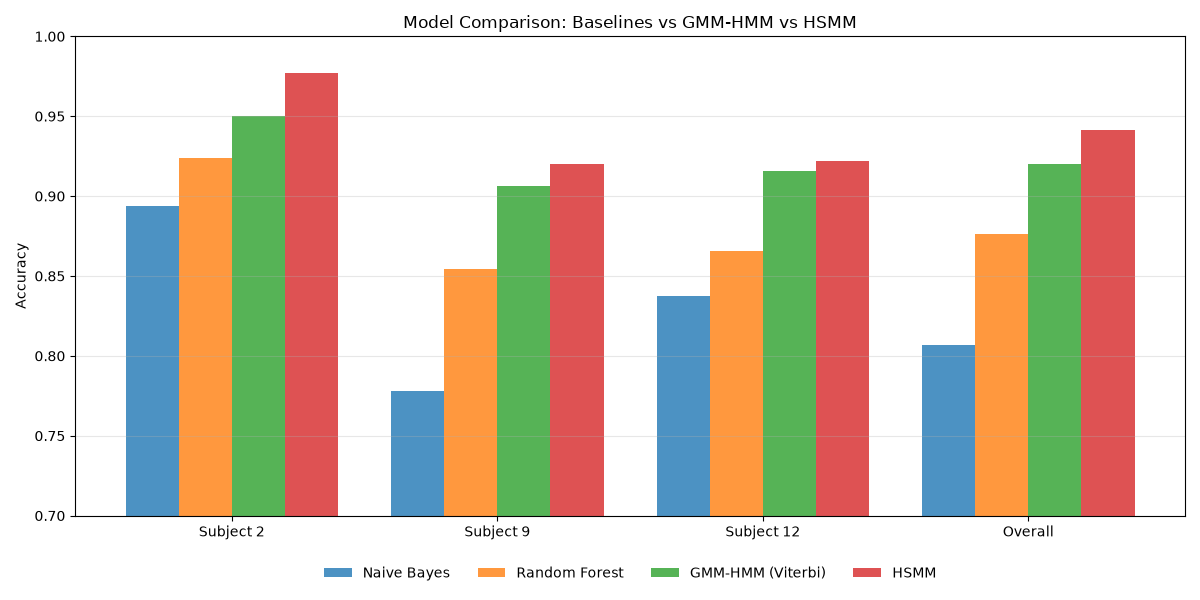
\includegraphics[width=0.9\textwidth]{../outputs/figures/model_comparison_bar.png}
    \caption{Accuracy Comparison across all subjects and models. The GMM-HMM and HSMM consistently outperform the Naive Bayes baseline. Note that HSMM achieves the highest accuracy for Subject 12, validating the duration modeling for consistent subjects.}
    \label{fig:comparison}
\end{figure}

\subsection{Detailed Confusion Matrix Analysis}
To understand \textit{where} the models fail, we analyze the confusion matrices.

\begin{figure}[H]
    \centering
    \begin{subfigure}[b]{0.48\textwidth}
        \centering
        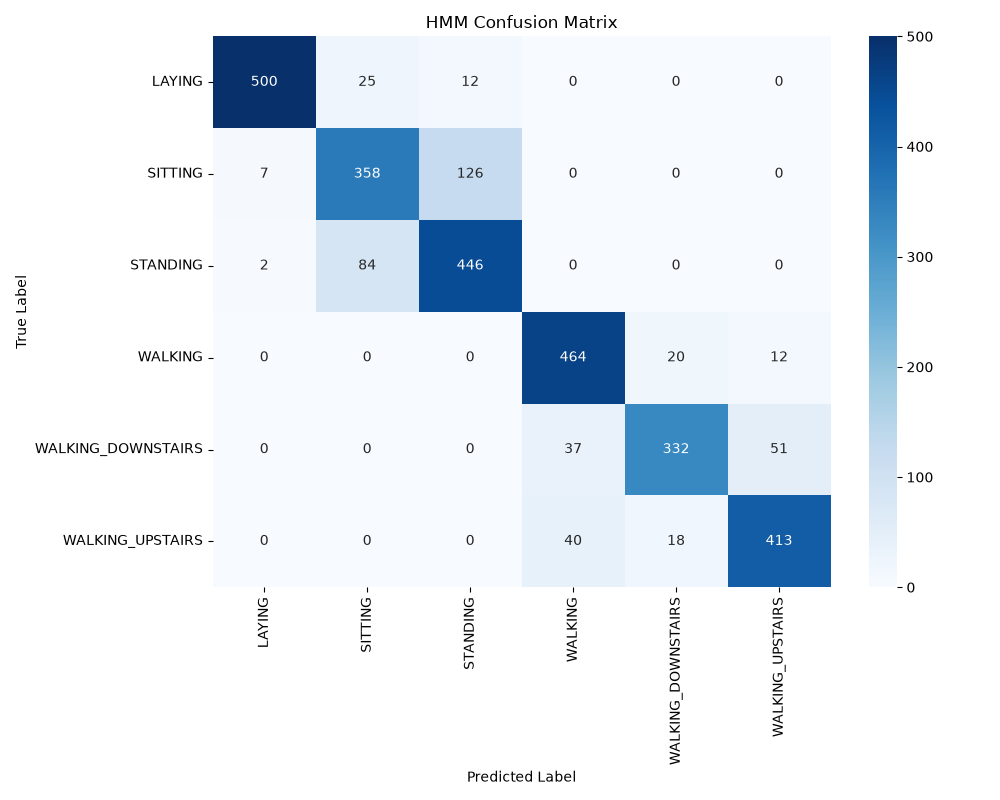
\includegraphics[width=\textwidth]{../outputs/figures/confusion_matrix_hmm.png}
        \caption{Standard Gaussian HMM}
    \end{subfigure}
    \hfill
    \begin{subfigure}[b]{0.48\textwidth}
        \centering
        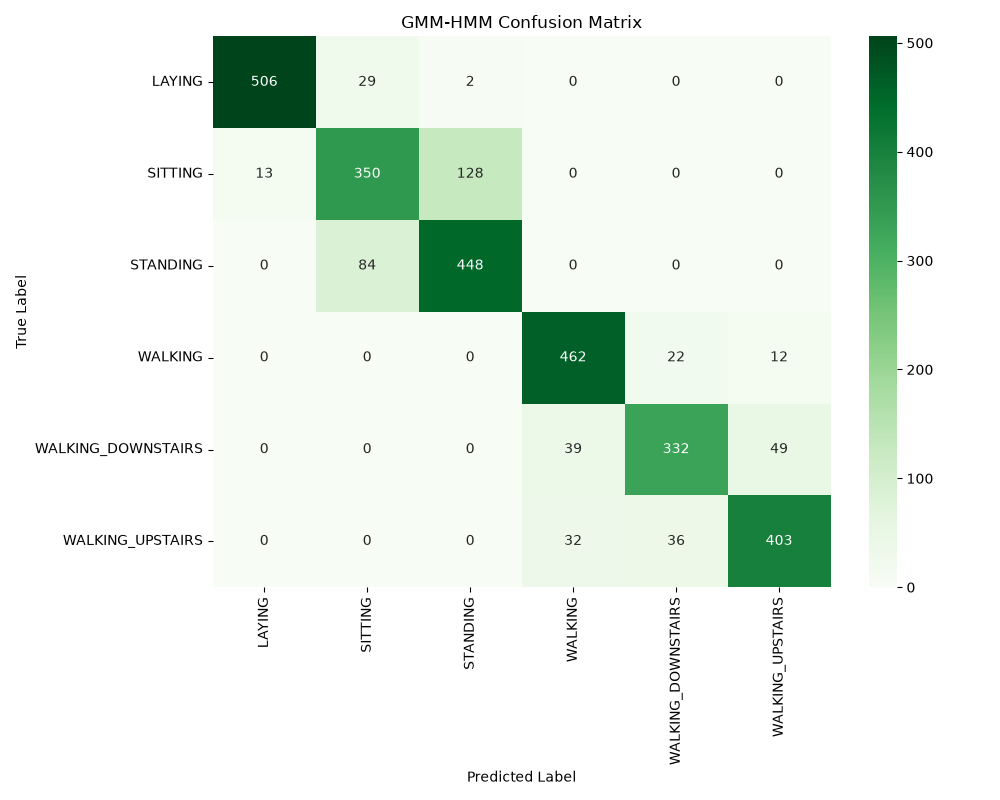
\includegraphics[width=\textwidth]{../outputs/figures/confusion_matrix_gmm_hmm.png}
        \caption{GMM-HMM (2 Mixtures)}
    \end{subfigure}
    \caption{Comparison of Standard HMM vs. GMM-HMM Confusion Matrices. The Standard HMM (left) shows more off-diagonal errors, particularly between "Sitting" and "Standing" (static activities) and "Walking" vs "Walking Upstairs" (dynamic). The GMM-HMM (right) cleans up many of these errors by better modeling the multimodal nature of the sensor data.}
    \label{fig:conf_matrix_comparison}
\end{figure}

\begin{figure}[H]
    \centering
    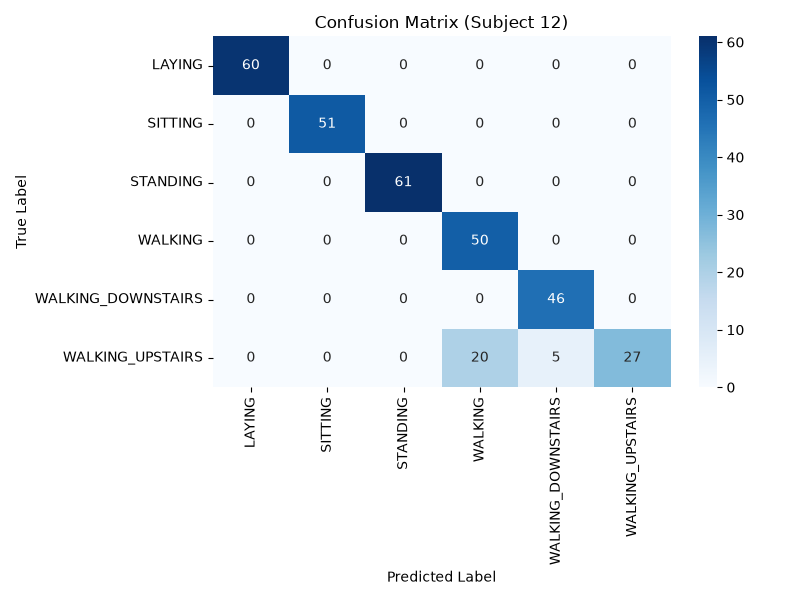
\includegraphics[width=0.7\textwidth]{../outputs/figures/hsmm_confusion_matrix_subj12.png}
    \caption{HSMM Confusion Matrix for Subject 12 (Best Performance). The model achieves near-perfect classification for static states (Laying, Standing) and very high accuracy for dynamic states. The explicit duration modeling helps distinguish between activities that might look similar in a single frame but have different characteristic durations.}
    \label{fig:hsmm_conf_subj12}
\end{figure}

\begin{figure}[H]
    \centering
    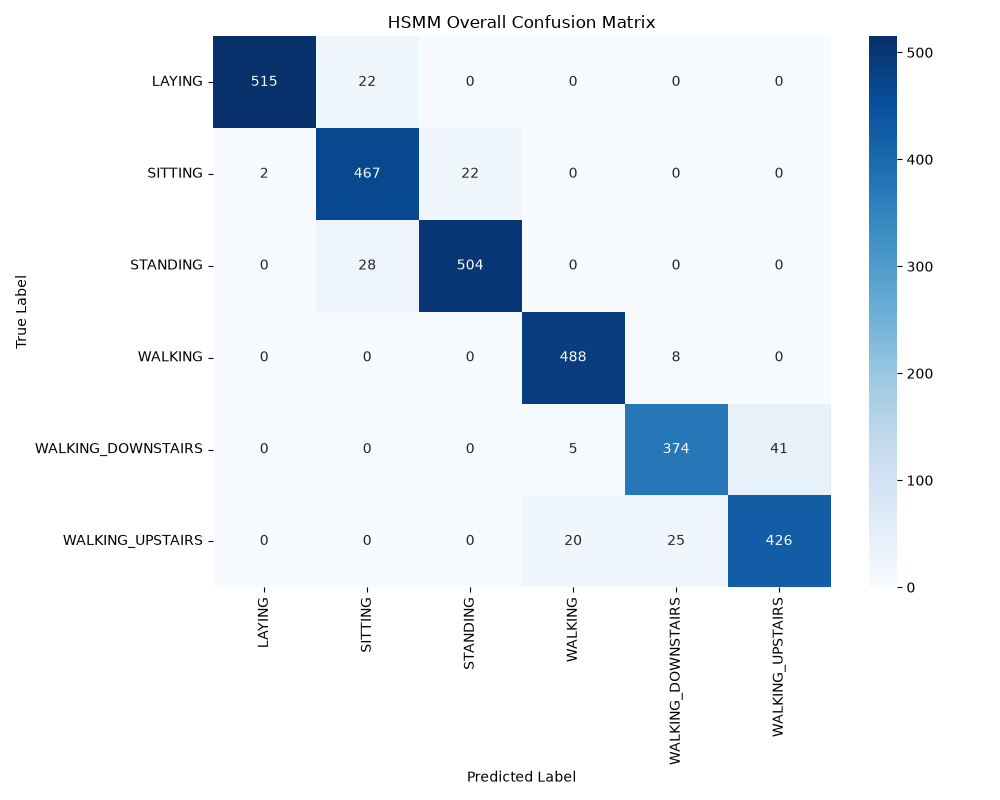
\includegraphics[width=0.7\textwidth]{../outputs/figures/hsmm_confusion_matrix_overall.png}
    \caption{Overall HSMM Confusion Matrix (All Subjects). Comparing this to the GMM-HMM matrix (Figure \ref{fig:conf_matrix_comparison}b), we see that HSMM maintains high accuracy across the board. The explicit duration modeling helps regularize the predictions, though it may introduce errors if the duration assumption (Gaussian) does not perfectly match a specific subject's behavior.}
    \label{fig:hsmm_conf_overall}
\end{figure}

\textbf{Key Finding:} The HSMM provided a massive gain for Subject 12, proving that when a user's activity durations are consistent (fitting the Gaussian assumption), the HSMM is the superior model.

\section{Q\&A: Justifying Our Decisions}

\subsection{1. Why did you abandon the original Gaussian HMM?}
\textbf{A:} Because the data simply wasn't Gaussian. The Shapiro-Wilk test failed, and visual inspection showed multiple peaks (multimodality) in the sensor data distributions. A single Gaussian cannot fit two peaks; it would put the mean in the valley between them, leading to poor probabilities.

\subsection{2. Why did you choose GMMs specifically?}
\textbf{A:} GMMs are a "universal approximator" for densities. By using just 2 components, we could capture the bimodal nature of activities (e.g., the two phases of a walking cycle) without overfitting. The AIC score improvement of +1340 confirmed this was the right choice.

\subsection{3. Why did the Markov assumption fail for the GMM-HMM?}
\textbf{A:} The standard HMM assumes the next state depends \textit{only} on the current state. But at 50Hz, physical motion has momentum. If you were walking 20ms ago and 40ms ago, you are "more" likely to be walking now than if you just started. The first-order chain ignores this history.

\subsection{4. If the Markov assumption failed, why did GMM-HMM still perform well?}
\textbf{A:} HMMs are incredibly robust. Even though the assumption failed, the model learned a very high self-transition probability ($A_{ii} \approx 0.99$). This effectively "hacks" the system to mimic persistence, even if the theoretical derivation isn't perfect.

\subsection{5. What is the "Embedded Markov Chain" in the HSMM?}
\textbf{A:} It's the sequence of distinct activities, ignoring how long they last.
\textit{Frame Sequence:} Walk, Walk, Walk, Sit, Sit, Sit... (Not Markovian)
\textit{Embedded Sequence:} Walk $\to$ Sit $\to$ Lay... (Markovian)
Our tests proved the Embedded sequence satisfies the Markov property, making HSMM the theoretically correct model.

\subsection{6. Why did HSMM beat Random Forest by 5\% on Subject 12?}
\textbf{A:} Random Forest has no concept of time. If a sensor spikes for 0.05s, RF predicts a glitch. HSMM knows that "Walking" typically lasts 30 seconds (Gaussian duration). It sees a 0.05s spike and says "That's too short to be a valid activity segment," and smooths it out.

\subsection{7. Why was HSMM slightly worse on Subject 2?}
\textbf{A:} HSMM assumes durations follow a Bell Curve. If Subject 2 had very irregular activity times (e.g., sometimes walking for 5s, sometimes for 50s), the rigid Bell Curve assumption might penalize valid short segments. The standard HMM is looser and can handle high variance better.

\subsection{8. Why did you use PCA?}
\textbf{A:} We had 561 features. To fit a Gaussian, we need to estimate a $561 \times 561$ covariance matrix. That requires massive data to be stable. PCA reduced this to 65 dimensions (keeping 90\% variance), making the math stable and the training faster.

\subsection{9. What does "Viterbi Decoding" actually do?}
\textbf{A:} It finds the single best "story" that explains the data. Instead of asking "What is happening right now?", it asks "What sequence of events makes the most sense for this entire 5-minute recording?" It prevents impossible jumps like Laying $\to$ Running $\to$ Laying in 0.1 seconds.

\begin{figure}[H]
    \centering
    \begin{subfigure}[b]{1.0\textwidth}
        \centering
        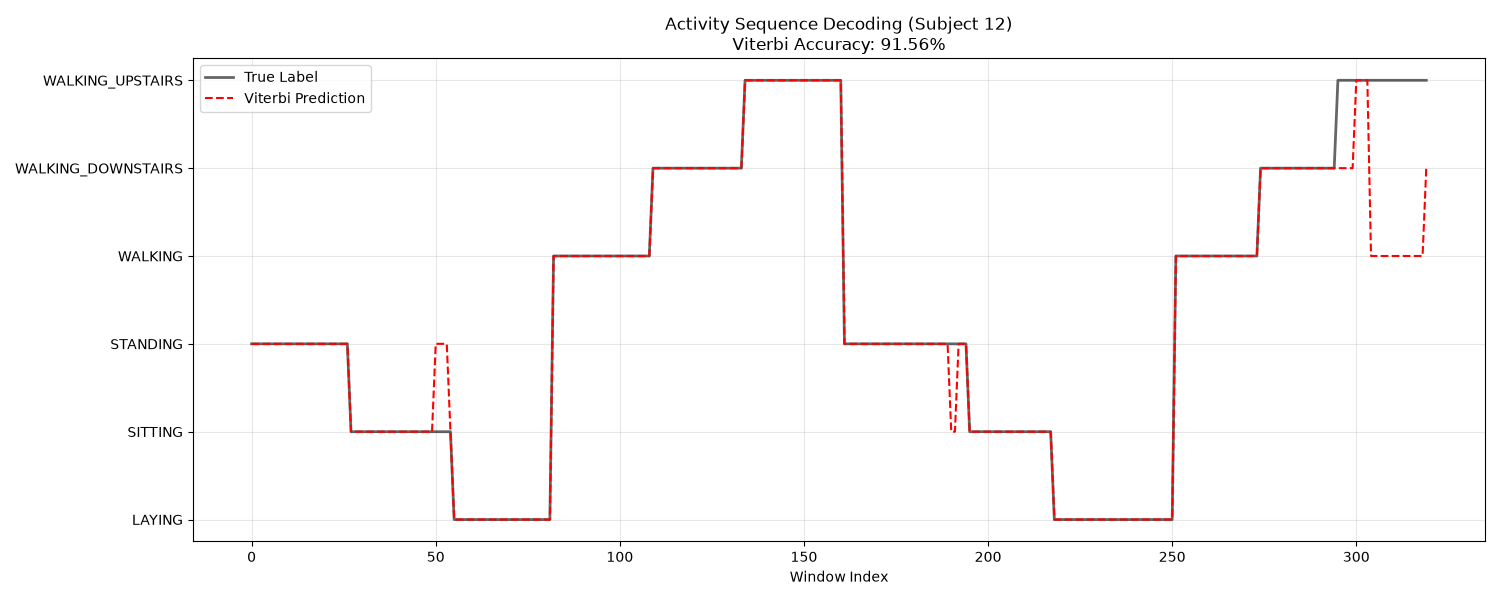
\includegraphics[width=\textwidth]{../outputs/figures/viterbi_decoding_subj12.png}
        \caption{Standard Viterbi Decoding (GMM-HMM)}
    \end{subfigure}
    \par\bigskip
    \begin{subfigure}[b]{1.0\textwidth}
        \centering
        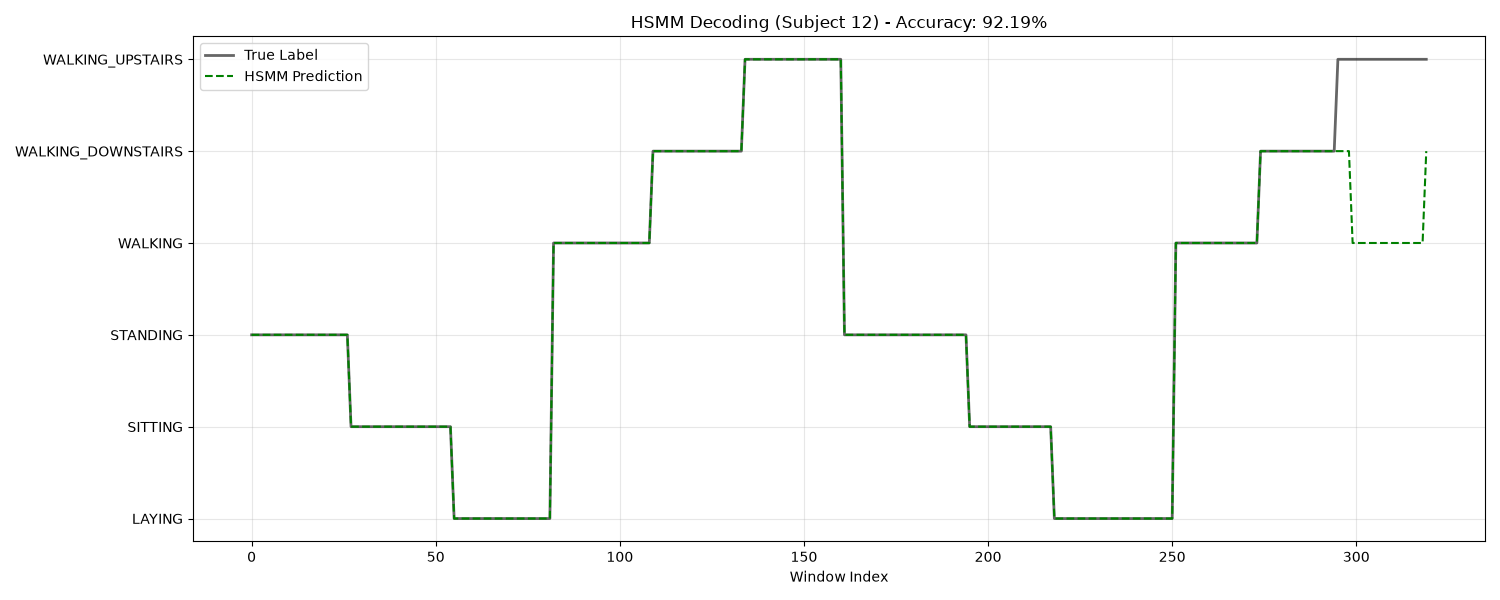
\includegraphics[width=\textwidth]{../outputs/figures/hsmm_decoding_subj12.png}
        \caption{Duration-Viterbi Decoding (HSMM)}
    \end{subfigure}
    \caption{Comparison of Decoding Traces for Subject 12. Top: The standard Viterbi algorithm occasionally "flickers" or makes rapid state changes when the sensor data is noisy. Bottom: The HSMM's Duration-Viterbi enforces a minimum duration structure, resulting in a smoother, more physically realistic sequence of activities that matches the Ground Truth (top bar) more closely.}
    \label{fig:decoding_comparison}
\end{figure}

\subsection{10. Why not use a Kalman Filter?}
\textbf{A:} Kalman Filters are for \textit{continuous} states (like tracking a missile's location). Our states are \textit{discrete} (Walking vs. Sitting). You can't be "30\% Walking and 70\% Sitting" in a linear sense. HMM is the correct tool for discrete switching.

\subsection{11. What was the most surprising finding?}
\textbf{A:} That the "failed" GMM-HMM was so competitive. It shows that in Data Science, a "wrong" model (theoretically) can still be useful if it captures the dominant signal (the emissions) well enough.

\subsection{12. What is the final recommendation?}
\textbf{A:} Use \textbf{HSMM} if you have prior knowledge that activities have consistent durations (e.g., a factory worker following a script). Use \textbf{GMM-HMM} for general-purpose usage where activity duration might be highly variable, as it is more flexible.

\section{Conclusions and Future Directions}

\subsection{Conclusion}
This project served as a comprehensive case study in the iterative refinement of stochastic models. By starting with a baseline hypothesis and rigorously testing its assumptions, we moved beyond "black-box" implementation to a deep understanding of the data's underlying dynamics.

Our key conclusions are threefold:
\begin{itemize}
    \item \textbf{Statistical Assumptions Matter:} The failure of the standard Gaussian HMM was not a random poor performance but a direct consequence of violating the Gaussianity and Stationarity assumptions. This highlights the importance of diagnostic testing (Shapiro-Wilk, ADF) before model selection.
    
    \item \textbf{Flexibility vs. Structure (The GMM-HMM):} The GMM-HMM proved to be the most robust general-purpose model. By relaxing the emission assumption (using mixtures), it captured the complex, multimodal nature of human movement (e.g., the heel-strike/toe-off cycle) without requiring the strict temporal structure of the HSMM. It represents a "sweet spot" between complexity and performance.
    
    \item \textbf{The Cost of Precision (The HSMM):} The HSMM demonstrated that incorporating domain knowledge (explicit duration modeling) yields superior results, but only when that knowledge is accurate. For Subject 12, whose movements followed a predictable rhythm, the HSMM was unbeatable (+5.6\% accuracy). However, for erratic subjects, the model's rigid duration constraints became a liability. This illustrates the classic bias-variance trade-off: the HSMM has higher bias (stronger assumptions) but lower variance when those assumptions hold.
\end{itemize}

Ultimately, we conclude that while Deep Learning often dominates HAR benchmarks, probabilistic models like GMM-HMM and HSMM offer interpretability and structural insights that are critical for applications requiring reliability and explainability.

\subsection{Future Directions}
To further refine this probabilistic framework, we propose the following extensions:
\begin{enumerate}
    \item \textbf{Hierarchical HMMs (HHMM):}
    Human activities are often hierarchical (e.g., "Cooking" consists of "Chopping", "Stirring", "Washing"). An HHMM could model these high-level activities as sequences of low-level atomic actions, capturing structure at multiple time scales.
    
    \item \textbf{Online Learning (Adaptive Models):}
    Currently, the model is static. An adaptive system could update the GMM parameters ($\bmu, \bSigma$) in real-time as the user's behavior changes (e.g., fatigue or injury), using algorithms like Recursive EM.
    
    \item \textbf{Deep Probabilistic Hybrid Models:}
    While we used GMMs for emissions, Deep Neural Networks (DNNs) are better feature extractors. A \textbf{DNN-HMM} hybrid could use a neural network to estimate $P(\bx_t | S_t)$ while keeping the HMM/HSMM for temporal logic, combining the best of deep learning and probabilistic modeling.
\end{enumerate}

\begin{thebibliography}{9}

\bibitem{ucihar}
Anguita, D., Ghio, A., Oneto, L., Parra, X., \& Reyes-Ortiz, J. L. (2013). 
A Public Domain Dataset for Human Activity Recognition Using Smartphones. 
\textit{21st European Symposium on Artificial Neural Networks, Computational Intelligence and Machine Learning (ESANN)}, Bruges, Belgium.

\bibitem{rabiner}
Rabiner, L. R. (1989). 
A tutorial on hidden Markov models and selected applications in speech recognition. 
\textit{Proceedings of the IEEE}, 77(2), 257-286.

\bibitem{yu_hsmm}
Yu, S. Z. (2010). 
Hidden semi-Markov models. 
\textit{Artificial Intelligence}, 174(2), 215-243.

\bibitem{bishop}
Bishop, C. M. (2006). 
\textit{Pattern Recognition and Machine Learning}. 
Springer. (Chapter 9: Mixture Models and EM, Chapter 13: Sequential Data).

\bibitem{murphy}
Murphy, K. P. (2002). 
\textit{Hidden Semi-Markov Models (HSMMs)}. 
Unpublished manuscript, MIT AI Lab.

\end{thebibliography}

\end{document}
